\section{Klassifikationsverfahren}\raggedbottom
Nachdem die Tweets vorbearbeitet, die Merkmale gewonnen und die Dimensionen zwecks verbesserter Performance reduziert wurden, können sie nun als Trainingsdatensatz für ein Klassifikationsverfahren verwendet werden. Im nachfolgenden Kapitel werden verschiedene solcher Verfahren vorgestellt und im Hinblick auf Voraussetzungen, Stärken und Schwächen analysiert. Ein besonderes Augenmerk soll in der Analyse auf die Kombination zwischen Algorithmus und den bereits erwähnten Methoden der Merkmalsextraktion gelegt werden, da erwartet wird, dass unterschiedliche Kombinationen sich qualitativ unterscheiden werden.  
\subsection{k-Nearest-Neighbor-Algorithmus}
Der k-Nearest-Neighbor-Algorithmus (KNN) ist eine parameterfreie Methode der Klassifikation (\textcolor{red}{Quelle}). Der zu klassifizierende Text wird zunächst analog zu den Trainingstexten vektorisiert. Über ein geeignetes Abstandsmaß werden nun die $k$ räumlich nächsten Nachbarn bestimmt. Der Text wird nun der Klasse zugeordnet, der die Mehrheit der Nachbarn angehören. Abbildung \ref{knn-alg} zeigt die k-Nearest-Neighbor-Klassifikation eines Punktes $x$ für $k=3$. Da die meisten Nachbarn hier dem Troll-Datensatz angehören, würde der zu $x$ gehörige Tweet somit als Troll-Tweet klassifiziert werden.\\
Die Wahl von $k$ ist entscheidend für die Qualität des Ergebnisses. Entscheidet man sich beispielsweise für ein zu kleines $k$, so ist möglich, dass vereinzelte Ausreißer die Genauigkeit trüben. Ist es auf der anderen Seite zu groß, so werden wahrscheinlich zu weit entfernte Punkte bei der Klassifikation miteinbezogen, was das Ergebnis wiederum verfälschen kann. Ferner ist bei Vorhandensein von 2 Klassen ein ungerades $k$ zu wählen, da andernfalls ein Unentschieden möglich ist.\\
\begin{figure}[htb]
	\begin{center}
		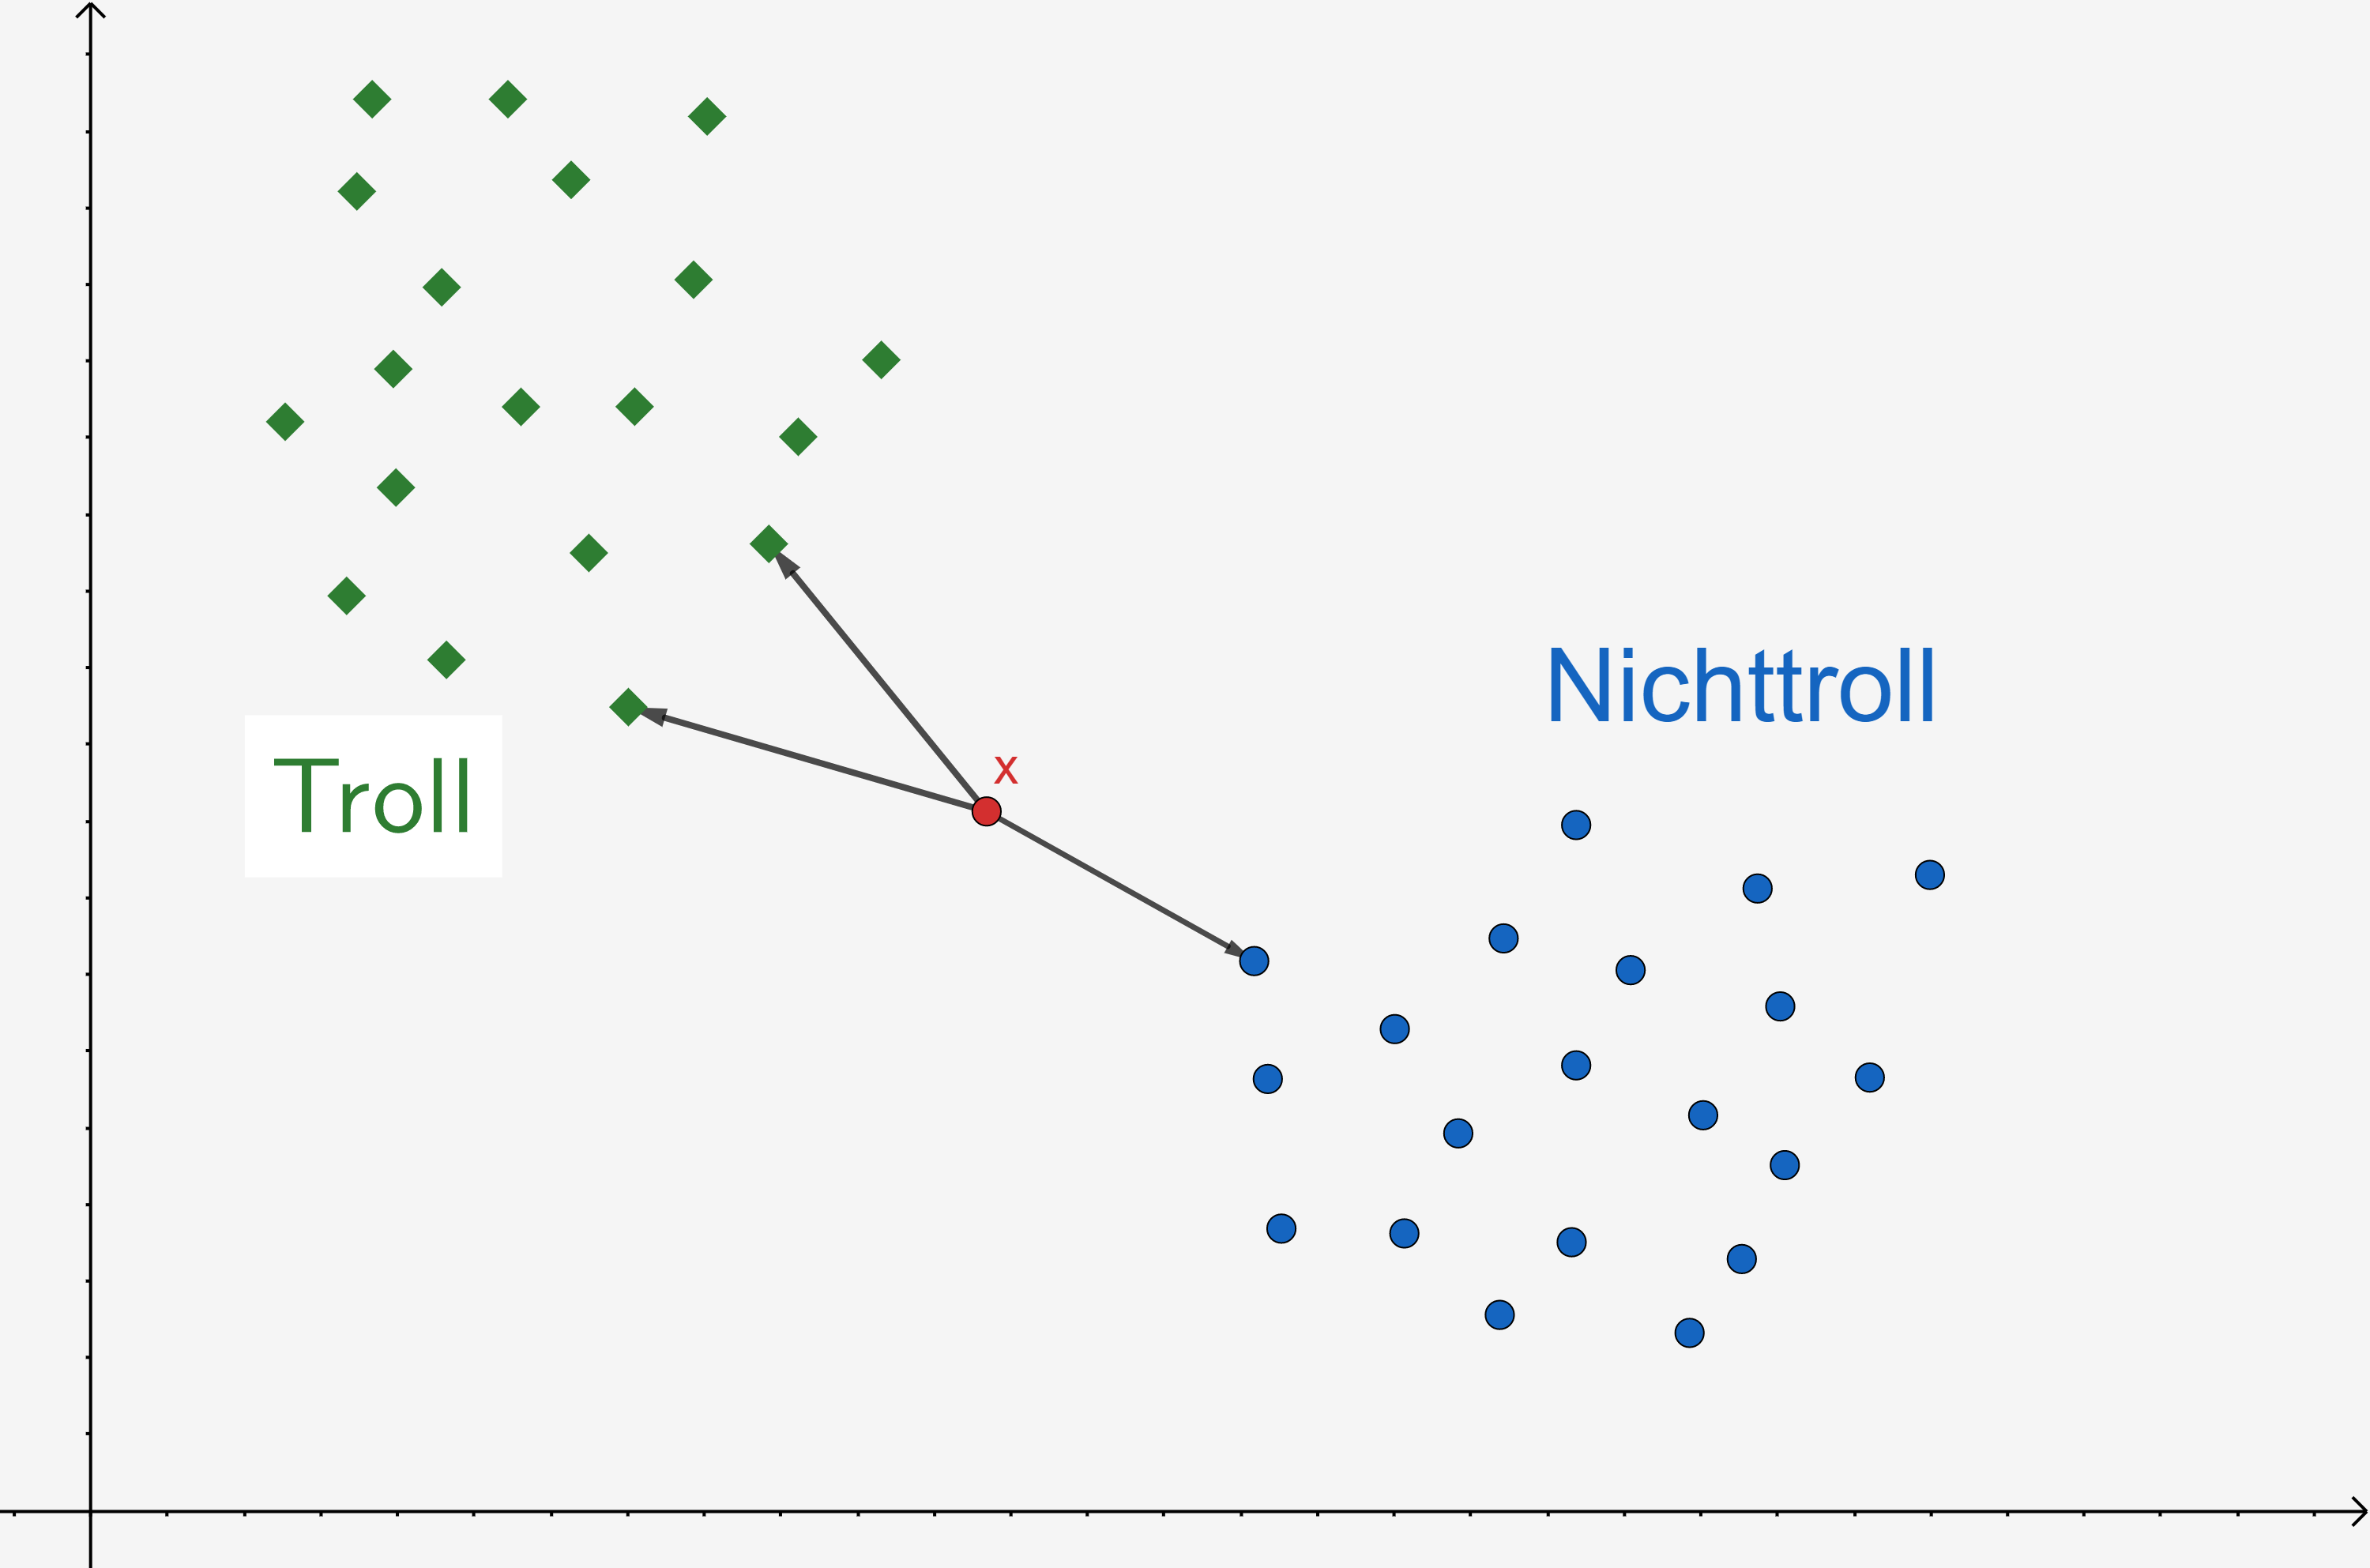
\includegraphics[scale=1.75]{bilder/Abb3.png}
		\caption{KNN-Klassifizierung für $k=3$}\label{knn-alg}
	\end{center}
\end{figure}\\
Eine zwingende Voraussetzung, um zuverlässig mit dem KNN-Algorithmus in diesem Projekt arbeiten zu können, ist die Dimensionalitätsreduktion. Die Merkmalsextraktion bringt bei den mehr als 600.000 Tweets hochdimensionale Vektoren hervor. Unbehandelt wären aufgrund der komponentenweisen Abstandsmessung Laufzeiten von einigen Minuten zu erwarten.\\
Die Vorteile dieses Verfahrens sind die einfache Implementierung und seine Eignung für alle möglichen Ausprägungen von Merkmalsräumen. Als Schwächen werden die bereits angesprochenen Probleme mit der Performance angesehen.
\subsection{Naiver Bayes-Klassifikator}
Der Naive Bayes-Klassifikator (NB) ist ein statistisches Verfahren der Klassifikation. Die Grundlage der Berechnung bildet hier der Satz von Bayes, bekannt aus der Wahrscheinlichkeitstheorie. In seiner herkömmlichen Interpretation beschreibt dieser die Berechnung der Wahrscheinlichkeit, dass ein Ereignis dem anderen vorausgegangen ist. Wendet man dies auf einen gegebenen Text $t \in T$ und die Klasse $k_i \in K$ an, so erhält man die Formel für die Wahrscheinlichkeit, dass $t$ der Klasse $k_i$ angehört (siehe Gleichung \ref{bayes}).
\begin{equation}
	P(k_i|t) = \frac{P(t|k_i) \cdot P(k_i)}{P(t)}
	\label{bayes}
\end{equation}
Der Klassifikator bestimmt nun diejenige Klasse $k_i$, für die der Wert dieser Formel maximal ist. Mathematisch formuliert:
\begin{equation}
	k = arg \max\limits_{k_i \in K} P(k_i|t) = arg \max\limits_{k_i \in K} \frac{P(t|k_i) \cdot P(k_i)}{P(t)}
\end{equation}
\pagebreak
\subsection{Support Vector Machine}
Lorem ipsum dolor sit amet.\pagebreak
\subsection{Weiteres Verfahren}
Lorem ipsum dolor sit amet.\pagebreak